\documentclass[border=3pt]{standalone}
% Preâmbulo compartilhado pelos diagramas TikZ da aula 13 (SLAM com EKF)
\usepackage[T1]{fontenc}
\usepackage[utf8]{inputenc}
\usepackage{lmodern}
\usepackage{amsmath}
\usepackage{xcolor}
\usepackage{tikz}
\usetikzlibrary{arrows.meta,angles,quotes,decorations.pathmorphing,decorations.pathreplacing,calc,
                positioning,shapes.geometric,shapes.misc,backgrounds,fit,
                math}

% Paleta (mesma dos SVGs originais)
\definecolor{dblue}{HTML}{2A5B8C}
\definecolor{dorange}{HTML}{B3541E}
\definecolor{dgreen}{HTML}{4A7C59}
\definecolor{dred}{HTML}{9C4B4B}
\definecolor{dcream}{HTML}{F4F1EA}
\definecolor{dshade}{HTML}{DDD7C9}

% Função gaussiana (não normalizada por padrão de escala visual)
\pgfmathdeclarefunction{gauss}{3}{%
  \pgfmathparse{1/(#3*sqrt(2*pi))*exp(-((#1-#2)^2)/(2*#3^2))}%
}

% Estilos comuns (prefixo d... para não colidir com chaves internas do pgf)
\tikzset{
  >={Stealth[length=2mm]},
  dguide/.style={gray!55, dashed, line width=0.4pt},
  daxis/.style={gray!60, line width=0.7pt, ->},
  dbody/.style={fill=black!3, draw=black!80, line width=1pt},
  dacc/.style={draw=dblue, line width=1pt},
  dlbl/.style={black!55, font=\small},
  dsub/.style={black!45, font=\footnotesize},
  dstate/.style={circle, draw=black!80, fill=dcream, line width=1pt,
                 minimum size=17mm, font=\large, inner sep=1pt},
  dobs/.style={circle, draw=black!80, fill=dshade, line width=1pt,
               minimum size=14mm, font=\large, inner sep=1pt},
  dbox/.style={rounded corners=2pt, draw=black!80, fill=dcream, line width=1pt,
               align=center, inner sep=6pt},
  dop/.style={circle, draw=black!80, fill=white, line width=1pt,
              minimum size=6mm, inner sep=0pt, font=\small},
  dtrans/.style={->, dblue, line width=1pt},
  dmeas/.style={->, dorange, line width=1pt},
  dcurve/.style={line width=1pt, dblue},
  dcurveb/.style={line width=1.4pt, dorange},
}

\begin{document}
\hyphenpenalty=10000 \exhyphenpenalty=10000 \tolerance=9999 \emergencystretch=3em
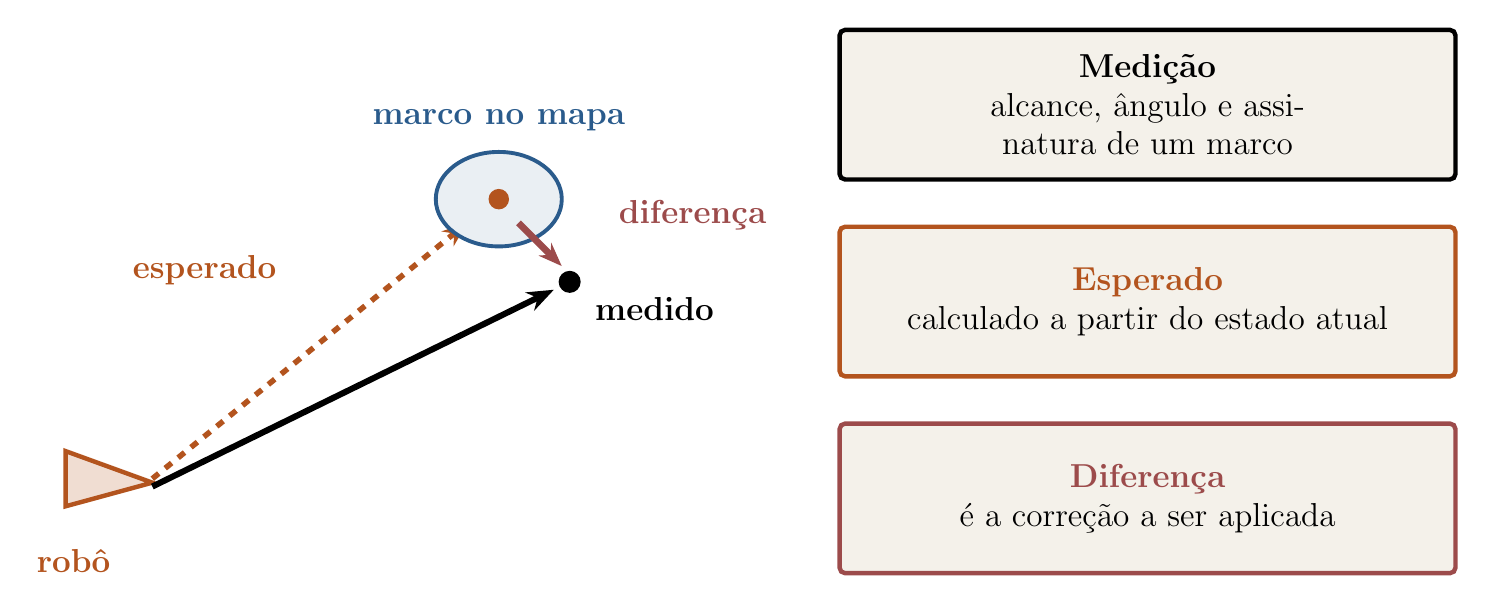
\begin{tikzpicture}[x=1cm,y=1cm]
\draw[dorange, fill=dorange!20, line width=1.6pt] (1.5,1.6) -- (2.6,1.9) -- (1.5,2.3) -- cycle;
\node[font=\large\bfseries, dorange] at (1.6,0.9) {robô};
\draw[dorange, dashed, line width=2pt, -{Stealth[length=3.2mm]}] (2.6,1.95) -- (6.6,5.2);
\draw[dblue, fill=dblue!10, line width=1.4pt] (7.0,5.5) ellipse (0.8 and 0.6); \fill[dorange] (7.0,5.5) circle (0.13);
\node[font=\large\bfseries, dorange, anchor=east, text width=3cm, align=right] at (4.3,4.6) {esperado};
\draw[black, line width=2.2pt, -{Stealth[length=3.4mm]}] (2.6,1.85) -- (7.7,4.35);
\fill[black] (7.9,4.45) circle (0.14);
\node[font=\large\bfseries, black, anchor=west] at (8.1,4.1) {medido};
\draw[dred, line width=2.4pt, -{Stealth[length=3mm]}] (7.25,5.2) -- (7.8,4.65);
\node[font=\large\bfseries, dred, anchor=west] at (8.4,5.3) {diferença};
\node[font=\large\bfseries, dblue] at (7.0,6.5) {marco no mapa};
\tikzset{b/.style={dbox, text width=7.4cm, minimum height=1.9cm, font=\large, line width=1.6pt, anchor=west}}
\node[b, draw=black] at (11.3,6.7) {\textbf{Medição}\\ alcance, ângulo e assinatura de um marco};
\node[b, draw=dorange] at (11.3,4.2) {\textbf{\textcolor{dorange}{Esperado}}\\ calculado a partir do estado atual};
\node[b, draw=dred] at (11.3,1.7) {\textbf{\textcolor{dred}{Diferença}}\\ é a correção a ser aplicada};
\end{tikzpicture}
\end{document}
